\documentclass[12pt,letterpaper]{article}

%%
%% Required packages:
%%
\usepackage{etex}
\usepackage{amsmath}
\usepackage{amssymb}
\usepackage{amstext}
\usepackage{amsthm}
\usepackage{fancyhdr,fancybox}
\usepackage{mathrsfs} % need for \mathscr command
\usepackage{multicol}
\usepackage[normalem]{ulem}
%\usepackage{pictex,pictexplus}
% \usepackage{pictexwd}
\usepackage{rotating}
\usepackage{url}
\usepackage{xfrac}
\usepackage{booktabs}
\usepackage{color,soul}
\usepackage{comment}

\usepackage{hyperref}
\hypersetup{
    colorlinks=true,     % false: boxed links; true: colored links
    linkcolor=blue,      % color of internal links
    citecolor=blue,      % color of links to bibliography
    filecolor=blue,      % color of file links
    urlcolor=blue        % color of external links
}


\usepackage{tikz}
\usetikzlibrary{backgrounds,calc}

%%
%% Common formatting commands
%%
\setlength{\parindent}{0in}
\setlength{\textwidth}{7in}
\setlength{\evensidemargin}{-0.25in}
\setlength{\oddsidemargin}{-0.25in}
\setlength{\parskip}{.5\baselineskip}
\setlength{\topmargin}{-0.5in}
\setlength{\textheight}{9in}

%               Problem and Part
\newcounter{problemnumber}
\newcounter{partnumber}
\newcounter{subpartnumber}
\newcommand{\Problem}{%
  \refstepcounter{problemnumber}%
  \setcounter{partnumber}{0}%
  \setcounter{subpartnumber}{0}%
  \item[\makebox{\hfil\textbf{\theproblemnumber.}\hfil}]%
  }
\newcommand{\InProblem}[2][1.6]{%
  \refstepcounter{problemnumber}%
  \setcounter{partnumber}{0}%
  \setcounter{subpartnumber}{0}%
  \textbf{\theproblemnumber.}\ \ \parbox[t]{#1in}{#2}%
}
\newcommand{\InSmallProblem}[1]{\InProblem[1.05]{#1}}
\newcommand{\NoProblem}[1]{%
  \mbox{\hfil\textbf{#1}\hfil}%
  }
\newcommand{\UnProblem}{%
  \refstepcounter{problemnumber}%
  \setcounter{partnumber}{0}%
  \setcounter{subpartnumber}{0}%
  \mbox{\hfil\textbf{\theproblemnumber.}\hfil}%
  }
\newcommand{\InFlexProblem}[1]{%
  \refstepcounter{problemnumber}%
  \setcounter{partnumber}{0}%
  \setcounter{subpartnumber}{0}%
  \textbf{\theproblemnumber.}\ \ #1%
}
%%  Part:
\newcommand{\Part}{%
  \renewcommand{\thepartnumber}{(\alph{partnumber})}%
  \refstepcounter{partnumber}
  \setcounter{subpartnumber}{0}%
  \item[(\alph{partnumber})]%
}
\newcommand{\InPart}[2][1.75]{%
  \renewcommand{\thepartnumber}{(\alph{partnumber})}%
  \refstepcounter{partnumber}%
  \setcounter{subpartnumber}{0}%
  (\alph{partnumber})\ \ \parbox[t]{#1in}{#2}%
}
\newcommand{\UnPart}{%
  \refstepcounter{partnumber}%
  \renewcommand{\thepartnumber}{(\alph{partnumber})}%
  \setcounter{subpartnumber}{0}%
  (\alph{partnumber})%
}
\newcommand{\InLargePart}[1]{\InPart[3.05]{#1}}
\newcommand{\InFullPart}[1]{\InPart[6.2]{#1}}
\newcommand{\InSmallPart}[1]{\InPart[1.05]{#1}}
%% SubPart:
\newcommand{\SubPart}{%
  \refstepcounter{subpartnumber}%
  \item[(\roman{subpartnumber})]%
  }
\newcommand{\InSubPart}[2][2.25]{%
  \stepcounter{subpartnumber}%
  (\roman{subpartnumber})\ \ \parbox[t]{#1in}{#2}%
}
\newcommand{\InSmallSubPart}[1]{\InSubPart[1.5]{#1}}
\newcommand{\InTinySubPart}[1]{%
  \stepcounter{subpartnumber}%
  (\roman{subpartnumber})\ \ \makebox{#1}%
}
\newcommand{\InMySubPart}[2][2.25]{%
  \stepcounter{subpartnumber}%
  \parbox[t]{#1in}{\makebox[0.3in][l]{(\roman{subpartnumber})}\ \ {#2}}%
}
\newcommand{\TrueFalse}{\textbf{T}\ \ \textbf{F}\ \ }
\newcommand{\TFPart}[1]{% 
  \stepcounter{partnumber}%
  \setcounter{subpartnumber}{0}%
  \item[(\alph{partnumber})] \TrueFalse\parbox[t]{5.5in}{#1}}

\newcommand{\Points}[1]{(#1 points) \ }
\newcommand{\Point}[1]{(#1 point) \ }


%% For Answers:
\newcounter{answernumber}
\newcommand{\Answer}{%
  \refstepcounter{answernumber}%
  \setcounter{partnumber}{0}%
  \setcounter{subpartnumber}{0}%
  \item[\makebox{\hfil\textbf{\theanswernumber.}\hfil}]%
  }


% Setting up the headers for the first page
%\chead{} % will default to what is typed in the file.
\fancyhead[L]{\textsc{Math 22a}}
\fancyhead[R]{\textsc{Fall 2024}}
\fancyfoot[R]{
	\vspace*{\fill}\footnotesize\textcopyright{} \emph{Harvard Math 22a}	
}
\renewcommand{\headrulewidth}{0pt}

%\fancyhead[C]{}
%	\chead{}	
%	\lhead{}
%	\rhead{}
%	\cfoot{}


% Putting copyright on the footer of each page
%\fancypagestyle{secondpage}{
%	\fancyhead[C]{TESTing again} % change this to be blank
%		%\chead{}	
%	\fancyhead[L]{bears} % change this to be blank
%	\fancyhead[R]{dogs} % change this to be blank
%	\fancyfoot[R]{ %keeps the footer the same
%		\vspace*{\fill}\footnotesize\textcopyright{} \emph{Harvard Math 22a}	
%	}
%}
%\renewcommand{\headrulewidth}{0pt}
%\pagestyle{fancy}
\pagestyle{empty}


%\lhead{}
%\rhead{}
%\rfoot{\vspace*{\fill}\footnotesize\textcopyright{} \emph{Harvard Math 22a}}
%\renewcommand{\headrulewidth}{0pt}
%\pagestyle{fancy}




%%
%% Common shortcut commands:
%%
\newcommand{\ds}{\displaystyle}
\newcommand{\sgn}{\operatorname{sgn}}
\renewcommand{\Pr}{\operatorname{P}}
\newcommand{\CPr}[3][{}]{\Pr_{\text{#1}}\left(#2\,|\,#3\right)}

\newcommand{\C}{\mathbb{C}}
\newcommand{\R}{\mathbb{R}}
\newcommand{\Z}{\mathbb{Z}}
\newcommand{\N}{\mathbb{N}}
\newcommand{\Q}{\mathbb{Q}}
\newcommand{\D}{\mathbb{D}}

\newcommand{\rref}{\operatorname{rref}}
\newcommand{\im}{\operatorname{im}}
\newcommand{\rank}{\operatorname{rank}}
\newcommand{\diag}{\operatorname{diag}}
\newcommand{\Span}{\operatorname{span}}
%\renewcommand{\vec}[1]{\mathbf{#1}}
\newcommand{\charpoly}{\mathscr{P}}
\newcommand{\nicefrac}[2]{\sfrac{#1}{#2}} % using xfrac package
\newcommand{\topology}{\mathcal{T}}
\newcommand{\Inn}{\operatorname{Inn}}

\newcommand{\blankbox}[2]{\fbox{\rule{#1}{0in}\rule{0in}{#2}}}

\newenvironment{myindentpar}[1]%
 {\begin{list}{}%
         {\setlength{\leftmargin}{#1}
          \setlength{\rightmargin}{\leftmargin}}%
         \item[]%
 }
 {\end{list}}
\newtheorem{theorem}{Theorem}
\newtheorem*{NStheorem}{Theorem}
\newtheorem{cor}[theorem]{Corollary}
\newtheorem*{claim}{Claim}
\newtheorem{defn}{Definition}

\newenvironment{amatrix}[1]{%
  \left(\begin{array}{@{}*{#1}{c}|c@{}}
}{%
  \end{array}\right)
}

%--------grstep
% For denoting a Gauss' reduction step.
% Use as: \grstep{\rho_1+\rho_3} or \grstep[2\rho_5 \\ 3\rho_6]{\rho_1+\rho_3}
\newcommand{\grstep}[2][\relax]{%
   \ensuremath{\mathrel{
       {\mathop{\longrightarrow}\limits^{#2\mathstrut}_{
                                     \begin{subarray}{l} #1 \end{subarray}}}}}}
\newcommand{\swap}{\leftrightarrow}



\usepackage{skak} % for chess!


\chead{\Large\textbf{Raisin Games}}

\begin{document}
\thispagestyle{fancy}

\begin{enumerate}
  \Problem Here is a simple game.  Start with a pile of raisins.  A
  turn consists of a player taking $1$, $2$, $3$ or $4$ raisins.  The
  last player to have a turn (that is, the player who takes the last
  raisin) wins.  Can you find an optimal strategy?  Who should win --
  the player who goes first or the player who goes second?
  \vfill

  \Problem
  Tweak the previous game to allow each player to take $1$ through $n$
  raisins.  How has the game changed?
  \vfill

  \Problem\label{prob:2piles}%
  Start with two piles of raisins.  A player's turn consists of taking
  \emph{either}\ some (any number of) raisins from a single pile
  \emph{or}\ the same number of raisins from both piles.  The person
  to take the last raisin wins.  Can you find an optimal strategy?
  \vfill
  \newpage



%  \Problem \textbf{The Homework's Raisin Game.} There is a competitive game
%  for two players that works as follows.  The game begins with a
%  handful of raisins split into two separate (and not necessarily
%  equal!) piles on the table.  The players alternate taking complete
%  turns until one of them is unable to take a complete turn; that
%  player loses the game.  A complete turn consists of two steps:
%  First, the player eats one of the piles on the table; Second, the
%  player divides the remaining pile into two new piles (of arbitrary
%  sizes, but non-empty), thus completing the turn.
%  \begin{enumerate} 
%    \Part Find some classmates to play with.  
%
%    \Part Play the game a few times with your classmates.  As we hinted
%    in class, start \emph{small}, and keep track of who wins which
%    games, Player 1 or Player 2.
%
%    \Part You will find that the winner depends very much on what the
%    initial configuration of raisins looks like (i.e. how many are in
%    each pile).  Make a conjecture: For what ``ideal'' configurations of
%    raisins does Player 1 have a winning strategy?  
%
%    \Part Use mathematical induction (from next class) to prove that your ``ideal
%    configuration'' indeed describes all winning positions for Player 1
%    (and also that all other configurations represent losing positions.
%    (You are free to assume that each player will play according to an
%    optimal winning strategy.)
%  \end{enumerate}

\end{enumerate}


%\end{document}


\newpage
\chead{\Large\textbf{Raisin Games Answers and Solutions}}
\lhead{}
\rhead{}
\thispagestyle{fancy}
\begin{enumerate}
  \Answer 
  It's clear that if there are $1$--$4$ raisins, the first player can
  win immediately.  This means that if there are $5$ raisins in the
  pile, player one must lose.  If there are $6$-$9$ raisins in the
  pile, then the next player to play can leave $5$ raisins and thus
  win.  If there are $10$ raisins left, the player to play is in a
  losing position and must leave $6$--$9$ raisins for the next
  player. 

  This continues and we have the following conclusion: A pile with a
  multiple of $5$ raisins is a losing position and the player to play
  must lose.  A pile of any other size is a winning position and the
  player to play can always leave the next player in a losing
  position.  The strategy is simply to take the appropriate number of
  reasons to leave the other player with a multiple of $5$ raisins.

  \Answer
  Here ``multiple of $5$ raisins'' becomes ``multiple of $n+1$
  raisins.''  The rest of the answer remains the same.

  \Answer We make a large table of positions and describe them as
  ``Winning'' or ``Losing'' depending on the prospects for the player
  to play.  See Table~\ref{table:prob3}.


  The analysis builds from basic cases.  If there is only one pile,
  then the player to play wins (simply take the remaining pile).  If
  there's one raisin in each pile, then again the player to play wins
  (simply take $1$ from each pile).  If there is $1$ in one pile and
  more than $1$ raisin in the other, then the player cannot
  immediately win.  In fact, if there are piles of $1$ raisin and $2$
  raisins -- let's call this position $(1,2)$ -- then the player to
  play loses (the player must leave their opponent in a winning
  position).  But this means $(2,N)$ (with $N>1$) and $(1,N)$ (with $N>2$) are
  \emph{winning}\ positions, as the player to play can leave a losing
  position $(1,2)$.  (Of course, $(N,N)$ is a winning position for any
  $N\ge1$, as the player to play can simply take all the raisins.)
  Now a simple corollary is that $(N,N+1)$ (for $N>1$) is a winning
  position, as we can leave $(1,2)$ by taking $N-1$ from both piles.

  What if there are at least $3$ raisins in each pile?  If the
  position is $(3,3)$, then winning is easy: take all the raisins.  If
  the position is $(3,4)$, then a winning strategy is to take $2$ from
  each pile and leave $(1,2)$.  But with $(3,5)$, the player to play
  must play and leave a winning position.  Thus this is a losing
  position.  But then $(3,N)$ (where $N>5$) becomes a winning
  position: take raisins from the second pile to leave $(3,5)$.  Thus
  this is a winning position.  Again a simple corollary is that
  $(N,N+2)$ (for $N>3$) is a winning position, as we can leave $(3,5)$
  by taking $N-3$ from both piles.

  If there are $4$ raisins in one pile and at least that many in the
  other, things are now easy.  From our discussions above, we've seen
  that $(4,4)$, $(4,5)$ and $(4,6)$ are winning positions.  Now
  $(4,7)$ is a losing position, as we must leave a winning position.
  But this leads to two consequences: $(4,N)$
  (where $N>7$) is a winning position (leave $(4,7)$ by taking $N-7$
  from the second pile) and $(N,N+3)$ is a winning position for $N>4$
  (take $N-4$ from both to leave $(4,7)$).

  We continue on in the table through piles of at least $8$
  raisins. 

  \begin{table}[htbp]
    \centering
    \begin{tabular}{ll}
      Position & Outcome \\ \toprule
      $(1,1)$ & Win: take all \\
      \hl{$(1,2)$} & Lose \\
      $(1,N)$, $N>2$ & Win: leave $(1,2)$ \\ \midrule
      %%%% 22222222222222222222222222222
      $(2,2)$ & Win: take all, or leave $(1,2)$ \\
      $(2,N)$, $N>1$ & Win: take $N-1$ to leave $(1,2)$ \\\midrule
      %%%% 33333333333333333333333333333
      $(3,3)$ & Win: take all \\
      $(3,4)$ & Win: take $(2,2)$ to leave $(1,2)$ \\
      \hl{$(3,5)$} & Lose \\
      $(3,N)$, $N>5$ & Win: take ($0,N-5)$ to leave $(3,5)$ \\\midrule
      %%%% 44444444444444444444444444444
      $(4,4)$ & Win: take all \\
      $(4,5)$ & Win: take $(3,3)$ to leave $(1,2)$ \\
      $(4,6)$ & Win: take $(1,1)$ to leave $(3,5)$ \\
      \hl{$(4,7)$} & Lose \\
      $(4,N)$, $N>7$ & Win: take $(0,N-7)$ to leave $(4,7)$\\\midrule
      % $(5,5)$ & Win: take all \\
      % $(5,6)$ & Win: take $(4,4)$ to leave $(1,2)$ \\
      % $(5,7)$ & Win: take $(1,0)$ or $(2,2)$ to leave $(4,7)$ or $(3,5)$ \\
      % $(5,8)$ & Win: take $(1,1)$ to leave $(4,7)$ \\
      % $(5,9)$ & Lose\\
      % $(5,N)$, $N>9$ & Win: take from the second pile to leave $(5,9)$\\\midrule
      %%%% 55555555555555555555555555555555555 
      $(5,N)$, $N\ge5$ & Win: take from the second pile to leave $(5,3) = (3,5)$\\\midrule
      %%%% 66666666666666666666666666666666666
      $(6,6)$ & Win: take all \\
      $(6,7)$ & Win: take $(2,0)$ or $(5,5)$ to leave $(4,7)$ or $(1,2)$ \\
      $(6,8)$ & Win: take $(3,3)$ to leave $(3,5)$ \\
      $(6,9)$ & Win: take $(2,2)$ to leave $(4,7)$ \\
      \hl{$(6,10)$} & Lose\\
      $(6,N)$, $N>10$ & Win: take from the second pile to leave $(6,10)$\\\midrule
      %%%% 77777777777777777777777777777777777 
      $(7,N)$, $N\ge7$ & Win: take from the second pile to leave $(7,4) = (4,7)$\\\midrule
      %%%% 88888888888888888888888888888888888
      $(8,8)$ & Win: take all \\
      $(8,9)$ & Win: take $(7,7)$ to leave $(1,2)$ \\
      $(8,10)$ & Win: take $(5,5)$ to leave $(3,5)$ \\
      $(8,11)$ & Win: take $(4,4)$ to leave $(4,7)$ \\
      $(8,12)$ & Win: take $(2,2)$ to leave $(6,10)$ \\
      \hl{$(8,13)$} & Lose\\
      $(8,N)$, $N>13$ & Win: take from the second pile to leave $(8,13)$\\\midrule
    \end{tabular}
    \caption{Optimal Strategy For Problem~\ref{prob:2piles}}
    \label{table:prob3}
  \end{table}


  Now we might begin to look for patterns. This game is called
  \href{https://en.wikipedia.org/wiki/Wythoff\%27s_game}{Wythoff's
    game} or Wythoff's Nim, as it is a variant of a very famous game
  called \href{https://en.wikipedia.org/wiki/Nim}{Nim}.  (Wythoff
  invented it, or at least popularized it, in the early twentieth
  century shortly after the winning strategy for Nim was published.)
  Here is a paper on ``simple'' strategies to win the game based on
  Fibonacci numbers:
  \href{http://ci.nii.ac.jp.ezp-prod1.hul.harvard.edu/openurl/query?rfe_dat=ncid\%2FAN10437727&rft.spage=53&rft.volume=9&rft.date=2002}{\emph{Simple
      Winning Strategies for Wythoff's Game}}\ by Takemasa Ooya and
  Jin Akiyama.  (This pair also wrote a paper on the relation of the
  Fibonacci numbers to other, similar games: \emph{Impact of binary
    and {F}ibonacci expansions of numbers on winning strategies for
    {N}im-like games}, International Journal of Mathematical Education
  in Science and Technology, Vol.\ 34, pp.\ 121--135.)
% @article {MR1958736,
%     AUTHOR = {Ooya, Takemasa and Akiyama, Jin},
%      TITLE = {Impact of binary and {F}ibonacci expansions of numbers on
%               winning strategies for {N}im-like games},
%    JOURNAL = {Internat. J. Math. Ed. Sci. Tech.},
%   FJOURNAL = {International Journal of Mathematical Education in Science and
%               Technology},
%     VOLUME = {34},
%       YEAR = {2003},
%     NUMBER = {1},
%      PAGES = {121--135},
%       ISSN = {0020-739X},
%      CODEN = {IJMEBM},
%    MRCLASS = {91A46 (11A63 11A67)},
%   MRNUMBER = {1958736},
%        DOI = {10.1080/00207390304849},
%        URL = {http://dx.doi.org/10.1080/00207390304849},
% }


  In the literature (see, for example, Eric Duch\^ene and Sylvain
  Gravier, \emph{Geometrical extensions of Wythoff's game}, Discrete
  Mathematics, Vol.\ 309, \#11, pp.\ 3595--3608, available
  \href{http://www.sciencedirect.com.ezp-prod1.hul.harvard.edu/science/article/pii/S0012365X07010710}{online}),
  the game is described geometrically as moving a queen on an infinite
  chessboard.  The squares on the board are indexed by two integers,
  starting at zero and increasing (so $(0,0)$, $(5,7)$ and so on).
  The position $(m,n)$ in our description is now a square on the
  chessboard, and the goal is to get to the square $(0,0)$.  The
  allowable moves correspond to moves by a queen down and/or to the
  left:
  \begin{center}
    \begin{tikzpicture}[x=10mm,y=10mm,>=latex]
      \foreach \k in {0,1,...,11} 
      {
        \draw[thin,black] (\k,0) -- (\k,11.3);
        \draw[thin,black] (0,\k) -- (11.3,\k);
      }
      \foreach \k in {0,1,...,10} 
      {
        \node at ({\k+0.5},-0.3) {$\k$};
        \node at (-0.3,{\k+0.5}) {$\k$};
      }
      \begin{scope}
        \clip (0,0) rectangle (11.3,11.3);
        \foreach \x in {0,2,...,10} {
          \foreach \y in {1,3,...,11} {
            \fill[yellow!50,opacity=0.5] (\x,\y) rectangle ({\x+1},{\y+1});
          }
        }
        \foreach \y in {0,2,...,10} {
          \foreach \x in {1,3,...,11} {
            \fill[yellow!50,opacity=0.5] (\x,\y) rectangle ({\x+1},{\y+1});
          }
        }
      \end{scope}
      \node at (7.5,4.5) {\Large\symqueen};
      \draw[ultra thick,blue,->] (7.5,4.2) -- (7.5,0.5);
      \draw[ultra thick,blue,->] (7.2,4.5) -- (0.5,4.5);
      \draw[ultra thick,blue,->] (7.3,4.3) -- (3.5,0.5);
      \draw[line width=4pt,red,->] (7.5,4.2) -- (7.5,3.2);
      \draw[line width=4pt,red,->] (7.2,4.5) -- (6.2,4.5);
      \draw[line width=4pt,red,->] (7.3,4.3) -- (6.65,3.65);
      % \node 
    \end{tikzpicture}
  \end{center}
  The original paper by Wythoff is in \emph{Nieuw archief voor
    wiskunde}\ on pages 199--202 of the 1905--1907 volume (available
  freely via
  \href{https://books.google.com/books?id=4ucKAAAAYAAJ}{Google
    books}).  He describes the $k$th losing position as $(\lfloor
  k\phi\rfloor, \lfloor k\phi^2\rfloor )$, where
  $\phi=\frac{1+\sqrt{5}}{2}$ is the golden ratio and $\lfloor
  x\rfloor$ is the ``floor'' (or integer part) of $x$.  (Of course
  these losing positions -- what Wythoff calls \emph{safe\
    combinations}, as in they are safe to leave for your opponent --
  are symmetric, so if $(a,b)$ is a losing position, so is $(b,a)$.
  We've implicitly assumed that $a<b$ in this description.)



\end{enumerate}
\end{document}


%%% Local Variables: 
%%% mode: latex
%%% TeX-master: t
%%% End: 
